
%(BEGIN_QUESTION)
% Copyright 2011, Tony R. Kuphaldt, released under the Creative Commons Attribution License (v 1.0)
% This means you may do almost anything with this work of mine, so long as you give me proper credit

An antimicrobial agent called {\it acrolein} used to protect diesel fuel from fungal growth may be manufactured by reacting propylene with steam and air in a reactor vessel: 

$$\includegraphics[width=15.5cm]{i01310x01.eps}$$

Suppose operators call you to troubleshoot a problem they are having with this process, and to help you start they show you this graphic display on one of their DCS workstations.  Identify the problem in this process, suggest at least two possible causes for it, and identify the next diagnostic step you would take to confirm the cause(s).

\vfil 

\underbar{file i01310}
\eject
%(END_QUESTION)





%(BEGIN_ANSWER)

This is a graded question -- no answers or hints given!

%(END_ANSWER)





%(BEGIN_NOTES)

The problem here is that propylene flow controller FC-203 is having trouble maintaining setpoint.

\vskip 10pt

Either there is very little propylene flow into the reactor (despite the controller trying to increase flow with a wide-open valve), or the transmitter is falsely indicating a very low flow rate.  The propylene supply header pressure (30 PSI) is barely above the reactor pressure (29 PSI), which would explain why we have very little flow through control valve FV-203 despite that valve being wide-open.  The problem most likely lies with the propylene system (not supplying enough pressure to this acrolein process), although if 30 PSI were a normal propylene supply pressure it could be that something downstream of the reactor is blocked causing the reactor's pressure to be abnormally high.  Without knowing whether 30 PSI is ``typical'' propylene pressure or 29 PSI is ``typical'' reactor pressure, we cannot tell for sure.  

If one were to overlook the low pressure differential between propylene supply and reactor pressure, a valid conclusion would be that perhaps control valve FV-203 isn't opening up as far as it should.

\vskip 10pt

A good ``next step'' would be to switch to another page on the DCS display and monitor parameters associated with propylene production and distribution.  

%INDEX% Process: acrolein production 
%INDEX% Process troubleshooting: diagnosing problem via DCS display

%(END_NOTES)


